\citeauthor{Munzner2014} answers many questions concerning the usage of visualisations in her book called ``Visualization Analysis and Design'' \iacite{Munzner2014}. This Chapter will discuss the most important answers because they are a necessity in understanding the questions of when, why and how to visualise. Furthermore, it introduces an analysis framework for visualisation tools in order to
put different tools in comparison.

From today's perspective with the ability to use artificial intelligence and machine learning, the question if we still need a human in order to create visualisations is valid. This question has a simple answer: if well-defined questions to ask about data exist in advance, it is possible to answer these purely with computational techniques from fields such as statistics and machine learning. If a solution to a problem has been fully automatised and has been deemed to be acceptable, there is no need for human judgement anymore and thus no need to design a visualisation tool. An example of a practical application would be the domain of stock market trading. A tool in that field can be fully automatised. There are currently many deployed systems for high-frequency trading. Those systems make decisions about buying and selling stocks when certain market conditions hold \iacite{Munzner2014}. Some other reasons where computers beat humans are mentioned below:
\begin{itemize}
\item Scale: Drawing a dataset of hundreds of thousands of items by hand is infeasible and would take a lot of time.
\item Efficiency: Once a problem has been solved with a computer it can be reused  indefinitely for different datasets and scenarios.
\item Quality: Precise data-driven rendering.
\end{itemize}
However, many analysis problems are poorly specified. Either the approach to the problem is unknown, or it is not obvious which questions the data could or should answer. In such a case, \citeauthor{Munzner2014} says, that the best path forward is an analysis process with a human in the loop \iacite{Munzner2014}. Even though there are a lot of use cases for a human in the loop, this paper only discusses one which deals with \ac{EDA} (see Chapter \ref{s:eda} on page \pageref{s:eda} for more information.), which is essential for this thesis. Exploratory analysis in scientific discovery is a common case of the need of a human. A long-term visualisation tool which could be developed is a tool with the goal of speeding up and improving user's ability to generate and check hypotheses \iacite{Munzner2014}.

% Maybe use ability matrix here

Another important question answered by \citeauthor{Munzner2014} is: why depend on vision? As Chapter \ref{s:definition} on page \pageref{s:definition} already mentions, a part of visualisation is based on exploiting the human visual system as a means of communication. A significant amount of visual information processing occurs in parallel through high-bandwidth channels to our brain. One example \citeauthor{Munzner2014} mentions is visual popout: one red item in a sea of gray ones is immediately noticed. This exploit of a human visual system can be used effectively to highlight specific information and to draw attention to a part of the visualisation.

Furthermore a single static view can show only one aspect of a dataset. This fact is already part of the answer of the next question: why use interactivity? Even though there are combinations of simple datasets and tasks where only a single visual encoding and therefore a single static view is needed, it does not apply for large complex datasets where interactivity allows to change displays and supports many possible queries. Interactivity could be used to investigate multiple levels of detail at once, ranging from a very specific detailed view of a small part to a very high-level summarization \iacite{Munzner2014}.

The main goal of a design of a visualisation is to satisfy rather than optimise. One of the many possible good solutions to a problem is much harder to find than one of the even larger number of bad ones. Yet the validation of satisfaction is very difficult because there are so many questions considering wheter a visualisation tool has met the design goals \iacite{Munzner2014}.

Furthermore considering at least three different kinds of limitations when designing or analysing visualisations is important:
\begin{enumerate}
\item computational capacity
\item human perceptual and cognitive capacity
\item display capacity
\end{enumerate}

All three limitations can be subsumed with the term scalability.

One of the most important questions \citeauthor{Munzner2014} answers is called: why analyse? In order to answer the question, she features an analysis framework that helps to think about design choices for visualisations systematically. Figure \ref{fig:an-framework} on page \pageref{fig:an-framework} shows the high-level framework she provides for analysing a visualisation's use according to three questions: what data does a user see, why does the user intend to use a visualisation tool and how are the visual encoding and interaction idioms constructed in terms of design choices \iacite{Munzner2014}.

\begin{figure}[!htb]
\centering
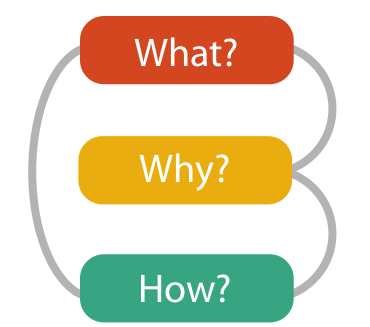
\includegraphics[width=0.3\textwidth,keepaspectratio]{images/basics/analysis-framework.png}
\caption[
    Three-part analysis framework for a visualisation instance: why is the task being performed, what data is shown in the views, and how is the visualisation idiom constructed in terms of design choices \iacite{Munzner2014}.
]{Three-part analysis framework for a visualisation instance: why is the task being performed, what data is shown in the views, and how is the visualisation idiom constructed in terms of design choices.}
\label{fig:an-framework}
\end{figure}

At this time, two out of three main questions for this Chapter have been solved. A visualisation should be made if there are no questions according to given data known in advance. If a visualisation is combined with \ac{EDA}, it emphasises knowledge construction over knowledge storage or information transmission, therefore answering the question why to visualise.

In order to answer the last main question of this Section, \citeauthor{Munzner2014} features Figure \ref{fig:how} on page \pageref{fig:how} which provides a preview of a set of design choices, with a high-level breakdown into four major classes:

\begin{enumerate}

\ditem{Encode} \hfill \\
This first part of the Figure deals with the encoding of how to arrange data spatially and shows five different choices:
    \begin{enumerate*}[label={(\arabic*)}]
    \item express values,
    \item separate,
    \item order and
    \item align regions and
    \item use given spatial data directly.
    \end{enumerate*}
Another important aspect this part features is the usage of nonspatial visual channels including color, size, angle, shape and so forth according to the type of attribute. These channels are explained in detail later in this Chapter.

\ditem{Manipulate} \hfill \\
The second part handles different approaches manipulating different aspects of the visualisation like changing any aspect of the view, selecting elements from within the view and navigating to change the viewpoint within the view.

\ditem{Facet} \hfill \\
The third part shows three different choices of how to facet data between views.

\ditem{Reduce} \hfill \\
The fourth part again mentions three different options for how to reduce the data shown.

\end{enumerate}

\begin{figure}[!hbt]
\centering
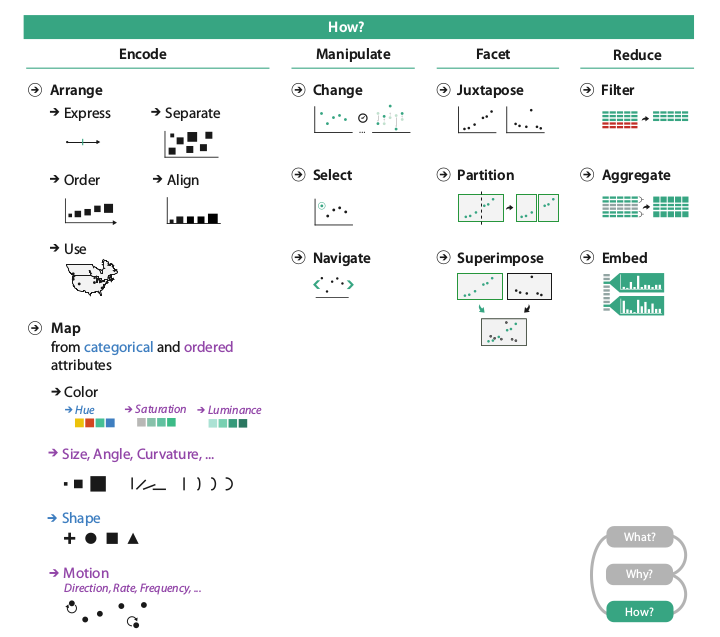
\includegraphics[height=10cm,keepaspectratio]{images/basics/how.png}
\caption[
    How to design visualisation idioms: encode, manipulate, facet, and reduce \iacite{Munzner2014}.
]{How to design visualisation idioms: encode, manipulate, facet, and reduce.}
\label{fig:how}
\end{figure}

Even though the main questions of this Section have been answered, one more question appeared in combination with the analysis framework: what? To summarise the usage of this framework, two more Figures are introduced: Figure \ref{fig:what} and \ref{fig:why} on page \pageref{fig:what} and \pageref{fig:why}.

\cbstart
Figure \ref{fig:what} starts with differentiating five different types of data (items, attributes, links, positions and grids) which is followed by dataset types consisting of different combinations of these data types. Considering a flat table as an example, the terms used in this thesis are the same as the ones \citeauthor{Munzner2014} uses. A row represents an item of data, whereas each column is an attribute of an item \iacite{Munzner2014}.
\cbend
The availability of these datasets can be either immediately in the form of a static file, or in the form of a data stream.

\begin{figure}[!htb]
\centering
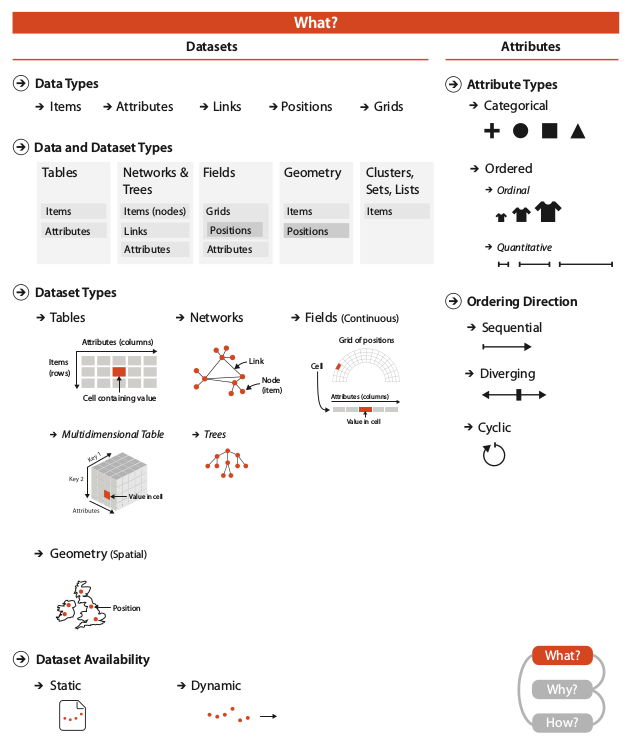
\includegraphics[height=10cm,keepaspectratio]{images/basics/what.png}
\caption[
    What can be visualised: data, datasets, and attributes \iacite{Munzner2014}.
]{What can be visualised: data, datasets, and attributes.}
\label{fig:what}
\end{figure}

Figure \ref{fig:why} is shown for the sake of completeness in combination with the analysis framework. It features two main parts: the reasons why a visualisation tool is being used (actions and targets). The highest-level actions to use visualisations are either to consume or produce information. The second-level action can be summarised as a search. From an abstract point of view, there is no difference in knowing the target or location a user is looking for or not. It ends up with either looking up that specific target or browsing and exploring the given visualisation in order to find it. At the low level, queries can be divided into three parts: identification of a specific target, comparison of multiple targets and the summarization of all targets.
The targets for all kinds of data are finding trends and outliers. This can be divided into two parts:
\begin{enumerate*}[label={(\arabic*)}]
\item finding one value, the extreme values or the distribution of all values for exactly one attribute, or
\item finding dependencies, correlations or similarities between multiple attributes.
\end{enumerate*}

\begin{figure}[!htb]
\centering
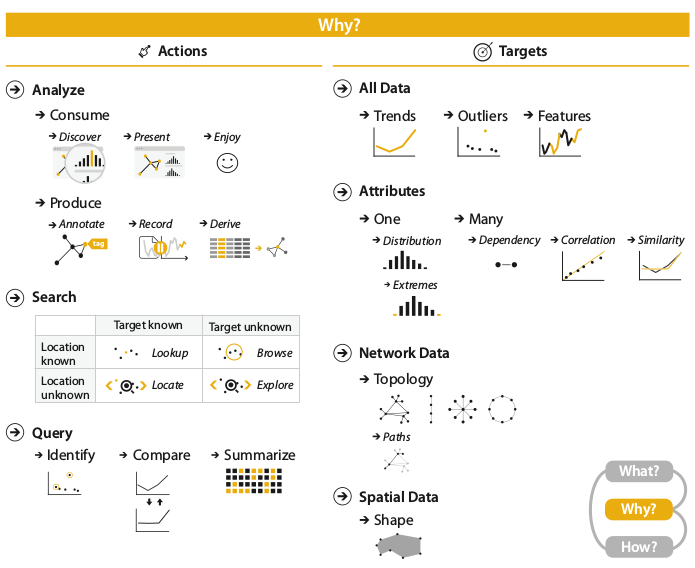
\includegraphics[height=10cm,keepaspectratio]{images/basics/why.png}
\caption[
    Why people are using visualisations in terms of actions and targets \iacite{Munzner2014}.
]{Why people are using visualisations in terms of actions and targets.}
\label{fig:why}
\end{figure}

The discussed framework will be used as a basis to analyse the related work mentioned in this thesis.

